%Autor: Simon Walker
%Version: 1.0
%Datum: 15.11.2019

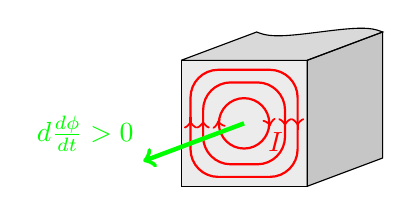
\begin{tikzpicture}[
x=8mm,
y=8mm,
z={(0.8*8mm, 0.3*8mm)},
]
	
	
	%%%%%%%%%%%%%%%%%%%%%%%%%%%%
	%Zylinder Farbig hinterlegen
	%%%%%%%%%%%%%%%%%%%%%%%%%%%%
	
	\filldraw [gray!15] (-1,-1,0) rectangle (1,1,0);
	\filldraw [gray!30] (-1,1,0) -- (1,1,0) -- (1,1,1.5) -- 
		plot[smooth, samples=25, variable=\t, domain=0:360]
		({1-(2*\t/360)},
		{1},
		{1.5+ 0.2*sin(\t)})
	-- (-1,1,1.5) -- (-1,1,0);
	\filldraw [gray!45] (1,-1,0) -- (1,1,0) -- (1,1,1.5) -- (1,-1,1.5) -- (1,-1,0);
	
	\draw (-1,-1,0) rectangle (1,1,0);
	\draw (-1,1,0) -- (1,1,0) -- (1,1,1.5) -- 
	plot[smooth, samples=50, variable=\t, domain=0:360]
	({1-(2*\t/360)},
	{1},
	{1.5+ 0.2*sin(\t)})
	-- (-1,1,1.5) -- (-1,1,0);
	\draw (1,-1,0) -- (1,1,0) -- (1,1,1.5) -- (1,-1,1.5) -- (1,-1,0);
	
	\draw [red, thick] (0, 0, 0) circle [radius=0.4];
	%\draw (x,y) arc (start:stop:radius);
	\draw[red, thick, -<] (170 : 0.4)  arc(170:190:0.4);
	\draw[red, thick, -<] (-10 : 0.4)  arc(-10:10:0.4);
	
	\draw [red, thick, rounded corners=10] (-0.65, -0.65, 0) rectangle (0.65, 0.65, 0);
	\draw [red, thick, -<] (-0.65, 0.1, 0) -- (-0.65, -0.08, 0);
	\draw [red, thick, -<] (0.65, -0.1, 0) -- (0.65, 0.08, 0);
	\draw [red, thick, rounded corners=10] (-0.85, -0.85, 0) rectangle (0.85, 0.85, 0);
	\draw [red, thick, -<] (-0.85, 0.1, 0) -- (-0.85, -0.08, 0);
	\draw [red, thick, -<] (0.85, -0.1, 0) -- (0.85, 0.08, 0);
	
	\node[red] at (0.5, -0.3, 0) {$I$};
	
	%\draw[red, thick, ->] (0,0 : 0.4)  arc[start angle=-10, end angle=0];
		
	\draw [green, ultra thick, ->] (0, 0, 0) -- (0, 0, -2);
	\node [above left, green] at (0, 0, -2) {$d\frac{d\phi}{dt}>0$};
      
      
%      %Hilfs Koordinaten System
%      \draw [->] (-3,0,0) -- (3,0,0);
%      \node [above] at (3,0,0) {x};
%      \draw [->] (0,-3,0) -- (0,3,0);
%      \node [above] at (0,3,0) {y};
%      \draw [->] (0,0,-3) -- (0,0,3);
%      \node [above] at (0,0,3) {z};
%   	
   
\end{tikzpicture}
